\section{NestJS}
\label{sec:nestjs}
NestJS é um framework em NodeJS de código aberto lançado em 2017 para o desenvolvimento de aplicações \textit{server-side}. Diante de outras tecnologias já consolidadas no JavaScript, esse \textit{framework} destaca-se por sua implementação base sustentar-se em elementos de programação orientada a objetos, programação funcional e programação reativa funcional para prover maior eficiência e escalabilidade.

Arquiteturalmente, para ser uma \textit{API RESTful} e aplicar o protocolo HTTPS, o NestJS não reinventa a roda e por baixo dos panos utiliza outros \textit{frameworks} consagrados no mercado, como o ExpressJS e Fastify, deixando a encargo do desenvolvedor decidir qual irá ser utilizado. Ao fazer isso, essa tecnologia também permite a utilização da ampla gama de bibliotecas auxiliares do NodeJS, adaptando-se facilmente às peculiaridades de cada projeto \cite{Mysliwiec2023}.

Além disso, de acordo com a comunidade, à nível de organização de código, NestJS inspira-se fortemente no framework \textit{front-end} Angular \cite{Passos2018}. Partindo disso, uma aplicação NestJS consiste em uma organização hierárquica de múltiplos módulos onde cada módulo é encarregado de um fragmento da aplicação, possuindo seus componentes, \textit{middlewares}, filtros, \textit{pipes} e protetores de rota.

Por fim, a tecnologia dispõe de sua própria interface de linha de comando, onde é possível inicializar a estrutura base do projeto além de também incluir de maneira simplificada novos módulos à aplicação \cite{Mysliwiec2023a}.

\begin{figure}[H]
    \centering
    \caption{Estrutura base de um projeto NestJS.}
    \label{fig:nestjs}
    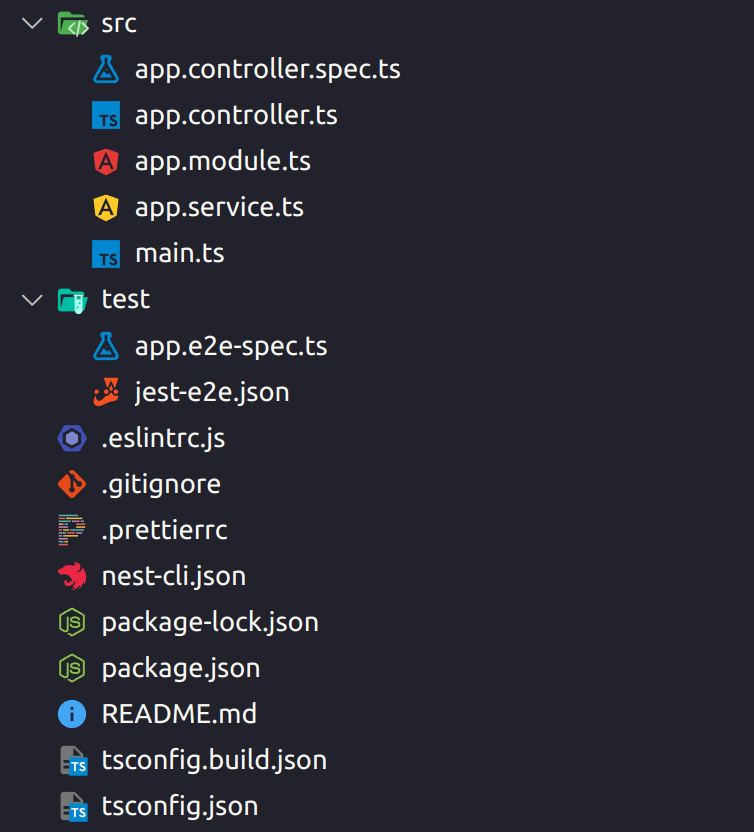
\includegraphics[width=.4\textwidth]{data/figures/nest.png}
    \fonte{Autor}
\end{figure}